\documentclass[tikz,border=8pt]{standalone}
% Shared look for every TikZ diagram. Load with \input{../../tools/tikz-style.tex}
\usepackage[T1]{fontenc}
\usepackage{lmodern}
\renewcommand{\sfdefault}{lmr}  % diagrams use the same serif as the text
\usetikzlibrary{arrows.meta, positioning, shapes.geometric, calc, fit, backgrounds}
\definecolor{cblue}{HTML}{4C78A8}
\definecolor{corange}{HTML}{F58518}
\definecolor{cgreen}{HTML}{54A24B}
\definecolor{cred}{HTML}{E45756}
\definecolor{cpurple}{HTML}{B279A2}
\definecolor{cgrey}{HTML}{6B6B6B}
\tikzset{
  every picture/.style={font=\sffamily, line width=1.2pt},
  box/.style={draw=#1, fill=#1!12, rounded corners=4pt, align=center, inner sep=7pt, minimum height=1.1cm},
  box/.default=cgrey,
  arrow/.style={-{Stealth[length=3mm]}, draw=cgrey, line width=1.4pt},
  title/.style={font=\sffamily\bfseries\Large},
  note/.style={font=\sffamily\small, text=cgrey, align=center},
}
\AtBeginDocument{\hyphenpenalty=10000 \exhyphenpenalty=10000}

\begin{document}
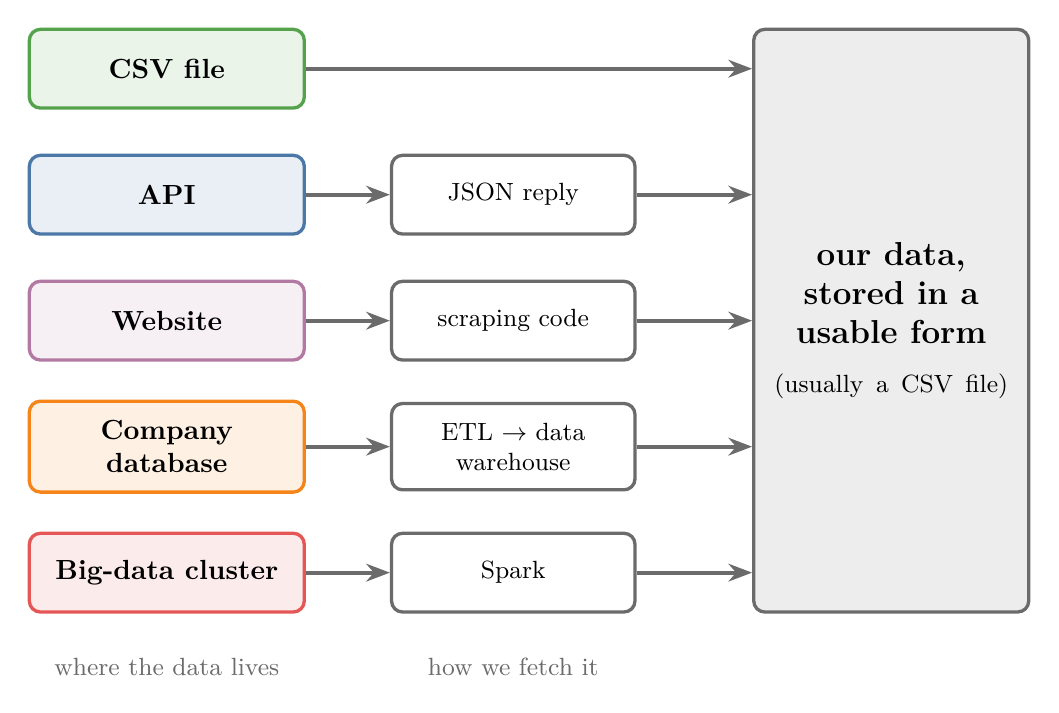
\begin{tikzpicture}[src/.style={box=#1, text width=3.0cm, minimum height=1.0cm, font=\sffamily\bfseries},
                    mid/.style={box=cgrey, fill=white, text width=2.6cm, minimum height=1.0cm, font=\sffamily\small}]
  \node[src=cgreen]  (csv) at (0,0)    {CSV file};
  \node[src=cblue]   (api) at (0,-1.6) {API};
  \node[src=cpurple] (web) at (0,-3.2) {Website};
  \node[src=corange] (db)  at (0,-4.8) {Company database};
  \node[src=cred]    (big) at (0,-6.4) {Big-data cluster};
  \node[mid] (json) at (4.4,-1.6) {JSON reply};
  \node[mid] (scr)  at (4.4,-3.2) {scraping code};
  \node[mid] (wh)   at (4.4,-4.8) {ETL $\to$ data warehouse};
  \node[mid] (sp)   at (4.4,-6.4) {Spark};
  \node[box=cgrey, text width=3.0cm, minimum height=7.4cm, font=\sffamily\bfseries\large] (ds) at (9.2,-3.2) {our data,\\stored in a usable form\\[4pt]\normalfont\small (usually a CSV file)};
  \draw[arrow] (csv) -- (csv -| ds.west);
  \foreach \a/\b in {api/json, web/scr, db/wh, big/sp} { \draw[arrow] (\a) -- (\b); \draw[arrow] (\b) -- (\b -| ds.west); }
  \node[note, text width=3.0cm] at (0,-7.6) {where the data lives};
  \node[note, text width=3.0cm] at (4.4,-7.6) {how we fetch it};
\end{tikzpicture}
\end{document}
